\section{Elektrotechnik}

\begin{defi}{Elektrische Ladung}
    Grundlegende Eigenschaft von Materie: [Q] = C (Coulomb)

    Ladung ist beobachtbar als nicht mit Gravitation erklärbare Kraftwirkung zwischen Materie.

    Körper mit gleicher Ladung stoßen sich ab.
    Ungleich geladene Körper ziehen sich an.

    $F$ ist definiert als Coulomb-Kraft:

    \[
        F = K \cdot \frac{Q_1 \cdot Q_2}{r^2} \cdot \vec{r}
    \]
\end{defi}

\begin{defi}{Arbeit}
    Potenzielle Energie: [W] = J (Joule)

    $W$ ist proportional zur Größe der bewegten Ladung $Q$.
    Energie, die als Ergebnis einer Ladungsträgerverschiebung bezogen auf die Ladungseinheit zur Verfügung:

    \[
        U = \frac{W}{Q}
    \]
\end{defi}

\begin{defi}{Spannung}
    Spannung: [U] = V (Volt)

    \[
        V = \frac{J}{C}
    \]

    In der Regel gibt man die Spannung eines Punktes immer in Bezug auf einen festen Nullpunkt an.
\end{defi}

\begin{defi}{Stromstärke}
    Gerichtete Bewegung in Ladungsträgern: [I] = A (Ampere)

    \[
        I = \frac{\Delta Q}{\Delta t}
    \]
\end{defi}

\begin{defi}{Widerstand}
    Widerstand gegen Ausgleichsbewegungen freier Ladungsträger: [R] = $\Omega$ (Omega)

    \[
        R = \frac{U}{I} =
        \begin{cases}
            \texttt{Reihenschaltung}   & \sum_{i = 1}^n R_i           \\
            \texttt{Parallelschaltung} & \sum_{i = 1}^n \frac{1}{R_i}
        \end{cases}
    \]

    Die Schaltsymbole sehen dabei wie folgt aus:

    \begin{center}
        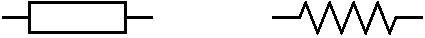
\includegraphics[width=0.35\textwidth]{includes/figures/defi_widerstand.pdf}
    \end{center}
\end{defi}

\begin{defi}{Kirchhoffsche Regeln}
    \begin{itemize}
        \item \emph{Knotenregel}:

              Die Summe aller zufließenden Ströme in einem Punkt ist gleich der Summe der abfließenden Ströme:

              \[
                  \sum_{i \in \{1, \ldots, n\}} I_{\text{in}_i} - \sum_{i \in \{1, \ldots, n\}} I_{\text{out}_i} \stackrel{!}{=} 0
              \]
        \item \emph{Maschenregel}:

              Die Summer aller abfallenden Spannungen in einem Schaltkreis ist gleich Null:

              \[
                  - U_Q + \sum_{i \in \{1, \ldots, n\}} U_i \stackrel{!}{=} 0
              \]
        \item \emph{Anwendungen}:
        \item \emph{Maschenstromverfahren}:
    \end{itemize}
\end{defi}

\begin{bonus}{Maschenstromverfahren}
    \begin{enumerate}
        \item Bestimmung der Anzahl Variablen

              $N$ (Anzahl der Zweige), $K$ (Anzahl der Knoten), $M$ (Anzahl Maschen)

              \[
                  M = N - K + 1
              \]
        \item Festlegung der Maschen
        \item Definition der Zweigströme
        \item Aufstellen der Gleichungssysteme mit der Maschenregel
        \item Ersetzen der Zweigspannungen mit Hilfe des Ohmschen Gesetzes und der Knotengleichung aus Schritt 3
    \end{enumerate}
\end{bonus}

\begin{example}{Maschenstromverfahren}
    \begin{center}
        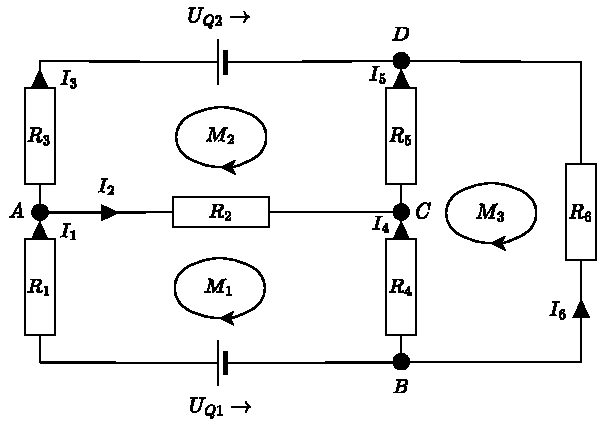
\includegraphics[width=0.65\textwidth]{includes/figures/example_maschenstromverfahren.pdf}
    \end{center}

    \begin{enumerate}
        \item Bestimmung der Anzahl Variablen:

              $N$ (Anzahl der Zweige), $K$ (Anzahl der Knoten), $M$ (Anzahl Maschen)

              \[
                  N = 6
              \]
              \[
                  K = 4
              \]
              \[
                  M = N - K + 1 = 6 - 4 + 1 = 3
              \]
        \item Festlegung der Maschen
        \item Definition der Zweigströme

              \[
                  \begin{matrix}
                      \phantom{-} \ I_1 & - \ I_3 &         & = & I_2 & \text{(Knoten A)} \\
                      - \ I_1           &         & - \ I_6 & = & I_4 & \text{(Knoten B)} \\
                                        & - \ I_3 & - \ I_6 & = & I_5 & \text{(Knoten D)}
                  \end{matrix}
              \]
        \item Aufstellen der Gleichungssysteme mit der Maschenregel

              \[
                  \begin{matrix}
                      U_1 & + \ U_2 &         & - \ U_4 &         &         & = &   & U_{Q1} & \text{(Masche 1)} \\
                          & - \ U_2 & + \ U_3 &         & - \ U_5 &         & = & - & U_{Q2} & \text{(Masche 2)} \\
                          &         &         & - \ U_4 & - \ U_5 & + \ U_6 & = &   & 0      & \text{(Masche 3)}
                  \end{matrix}
              \]
        \item Ersetzen der Zweigspannungen mit Hilfe des Ohmschen Gesetzes und der Knotengleichung aus Schritt
    \end{enumerate}

    \[
        \begin{matrix}
            R_1 \cdot I_1 & + \ R_2 \cdot (I_1 - I_3) &                   & + \ R_4 \cdot (I_1 + I_6) &                           &                   & = &   & U_{Q1} \\
                          & - \ R_2 \cdot (I_1 - I_3) & + \ R_3 \cdot I_3 &                           & + \ R_5 \cdot (I_3 + I_6) &                   & = & - & U_{Q2} \\
                          &                           &                   & + \ R_4 \cdot (I_1 + I_6) & + \ R_5 \cdot (I_3 + I_6) & + \ R_6 \cdot I_6 & = &   & 0
        \end{matrix}
    \]
\end{example}

\begin{example}{Maschenstromverfahren}
    \[
        \begin{matrix}
            I_1 \cdot & (R_1 + R_2 + R_3) & + \ I_3 \cdot & (- R_2)           & + \ I_6 \cdot & R_4               & = &   & U_{Q1} \\
            I_1 \cdot & (- R_2)           & + \ I_3 \cdot & (R_2 + R_3 + R_5) & + \ I_6 \cdot & R_5               & = & - & U_{Q2} \\
            I_1 \cdot & R_4               & + \ I_3 \cdot & R_5               & + \ I_6 \cdot & (R_4 + R_5 + R_6) & = &   & 0
        \end{matrix}
    \]

    Erstelle das zu lösende Gleichungssystem mit Widerstandsmatrix als Koeffizientenmatrix:

    Gegeben sind die folgenden Widerstände und Spannungen:

    \begin{center}
        \begin{tabular}{ccc}
            $R_1 = 10\Omega$  & $R_4 = 10\Omega$ & $U_{Q1} = 12V$  \\
            $R_2 = \ 5\Omega$ & $R_5 = 15\Omega$ & $U_{Q1} = \ 6V$ \\
            $R_3 = 15\Omega$  & $R_6 = 30\Omega$ &
        \end{tabular}
    \end{center}

    \[
        \begin{array}{cccc}
            R & I & = & U        \\\\
            \begin{pmatrix}
                R_1 + R_2 + R_3 & - \ R_2         & R_4             \\
                - \ R_4         & R_2 + R_3 + R_5 & R_5             \\
                R_4             & R_5             & R_4 + R_5 + R_6
            \end{pmatrix}
              &
            \begin{pmatrix}
                I_1 \\
                I_3 \\
                I_6
            \end{pmatrix}
              & = &
            \begin{pmatrix}
                \phantom{-} \ U_{Q1} \\
                - \ U_{Q2}           \\
                \phantom{-} \ \ 0
            \end{pmatrix} \\
            \begin{pmatrix}
                10 + 5 + 10 & - \ 5       & 10          \\
                - \ 5       & 5 + 15 + 15 & 15          \\
                5           & 15          & 5 + 15 + 30
            \end{pmatrix}
              &
            \begin{pmatrix}
                I_1 \\
                I_3 \\
                I_6
            \end{pmatrix}
              & = &
            \begin{pmatrix}
                \phantom{-} \ 12 \\
                - \ \ 6          \\
                \phantom{-} \ \ 0
            \end{pmatrix}     \\
            \begin{pmatrix}
                25    & - \ 5 & 10 \\
                - \ 5 & 35    & 15 \\
                5     & 15    & 50
            \end{pmatrix}
              &
            \begin{pmatrix}
                I_1 \\
                I_3 \\
                I_6
            \end{pmatrix}
              & = &
            \begin{pmatrix}
                \phantom{-} \ 12 \\
                - \ \ 6          \\
                \phantom{-} \ \ 0
            \end{pmatrix}     \\
            \begin{pmatrix}
                25    & - \ 5 & 10 \\
                - \ 5 & 35    & 15 \\
                5     & 15    & 50
            \end{pmatrix}
              &
            \begin{pmatrix}
                \phantom{-} \ 0.4941 \\
                - \ 0.0706           \\
                - \ 0.0706
            \end{pmatrix}
              & = &
            \begin{pmatrix}
                \phantom{-} \ 12 \\
                - \ \ 6          \\
                \phantom{-} \ \ 0
            \end{pmatrix}
        \end{array}
    \]

    Daraus ergibt sich:

    \[
        \begin{matrix}
            I_1 = &                         &   &                                   &   & \phantom{-} \ 0.4941 A \\
            I_2 = & \phantom{-} \ I_1 - I_3 & = & \phantom{-} \ 0.4941 A + 0.0706 A & = & - \ 0.5647 A           \\
            I_3 = &                         &   &                                   &   & - \ 0.0706 A           \\
            I_4 = & - I_1 - I_6             & = & - \ 0.4941 A + 0.0706 A           & = & - \ 0.4235 A           \\
            I_5 = & - I_3 - I_6             & = & \phantom{-} \ 0.0706 A + 0.0706 A & = & \phantom{-} \ 0.1412 A \\
            I_6 = &                         &   &                                   &   & - \ 0.0706 A           \\
        \end{matrix}
    \]
\end{example}